\documentclass[10pt,twocolumn]{article}

\usepackage[margin=0.75in]{geometry}
\usepackage{times}
\usepackage{microtype}
\usepackage{graphicx}
\usepackage{booktabs}
\usepackage{amsmath}
\usepackage{enumitem}
\usepackage{natbib}
\usepackage[hidelinks]{hyperref}
\usepackage{tcolorbox}
\usepackage{xcolor}
\usepackage{tikz}
\usepackage{tabularx}
\urlstyle{same}

% ── Flag macros (TikZ inline) ─────────────────────────────────────────────────
\newcommand{\flagCH}{%
\tikz[baseline=-0.55ex, x=1em, y=1em]{
  \fill[red!85!black] (0,0) rectangle (1.15,0.8);
  \fill[white] (0.48,0.14) rectangle (0.67,0.66);
  \fill[white] (0.25,0.305) rectangle (0.90,0.495);
}}
\newcommand{\flagBE}{%
\tikz[baseline=-0.55ex, x=1em, y=1em]{
  \fill[black] (0,0) rectangle (0.38,0.8);
  \fill[yellow!85!orange] (0.38,0) rectangle (0.76,0.8);
  \fill[red!80!black] (0.76,0) rectangle (1.15,0.8);
}}
\newcommand{\flagBA}{%
\tikz[baseline=-0.55ex, x=1em, y=1em]{
  \fill[blue!70!black] (0,0) rectangle (1.15,0.8);
  \fill[yellow!90!orange] (0.43,0.8) -- (1.15,0.8) -- (1.15,0.0) -- cycle;
  \foreach \x/\y in {0.43/0.72,0.52/0.62,0.61/0.52,0.70/0.42,0.79/0.32,0.88/0.22,0.97/0.12}{
    \node[white, scale=0.22] at (\x,\y) {$\star$};
  }
}}
\newcommand{\flagGB}{%
\tikz[baseline=-0.55ex, x=1em, y=1em]{
  \fill[blue!70!black] (0,0) rectangle (1.15,0.8);
  \draw[white, line width=0.19em] (0,0) -- (1.15,0.8);
  \draw[white, line width=0.19em] (0,0.8) -- (1.15,0);
  \draw[red!85!black, line width=0.09em] (0,0) -- (1.15,0.8);
  \draw[red!85!black, line width=0.09em] (0,0.8) -- (1.15,0);
  \fill[white] (0,0.29) rectangle (1.15,0.51);
  \fill[white] (0.46,0) rectangle (0.69,0.8);
  \fill[red!85!black] (0,0.34) rectangle (1.15,0.46);
  \fill[red!85!black] (0.515,0) rectangle (0.635,0.8);
}}

\setlength{\columnsep}{0.25in}
\setlength{\parindent}{1em}
\setlength{\parskip}{0pt}
\raggedbottom

\title{\textbf{Cross-Constituency Aggregation for Community Notes}}

\author{
Emrecan Ulu\\
University of Konstanz
\and
Jingyao\\
University of Konstanz
}

\date{}

\begin{document}

\maketitle

\begin{abstract}
Community Notes is X's crowd-based fact-checking system: contributors write
contextual notes, other contributors rate them, and a bridging algorithm decides
which notes become visible. The algorithm is designed to avoid simple majority
capture by estimating note quality separately from ideological alignment, so a
note should gain support across disagreement rather than only within one side
\citep{wojcik2022birdwatch,xcommunitynotes2026ranking}. This design is powerful,
but it also creates a visibility problem. Because the system works through
sparse and unequal participation, display decisions can depend heavily on the
ratings supplied by a relatively small active core, and many notes remain in
Needs More Ratings when the algorithm does not find enough diverse support
\citep{goyal2026qsmf,razuvayevskaya2025timeliness}. We argue that this is not
only a data-sparsity problem. It is also an aggregation problem: Community Notes
treats cross-group agreement indirectly, through a fitted model, rather than as
an explicit decision rule over constituencies.

We take inspiration from political science and social choice. In systems such
as Switzerland's double-majority referendum rule, important decisions must gain
support not only from a national majority but also from a majority of cantons;
the system treats cross-group support as part of the decision's legitimacy. Our
philosophy is simple: a note should not become visible because one active group
overwhelms the rest; it should become visible when each relevant constituency
has a real chance to support it. We operationalize this idea as
cross-constituency aggregation. We recover behavioral constituencies from
co-rating patterns among 200,000 active raters, compute each note's approval
rate inside each constituency, and combine those rates with a geometric mean
under a minimum-coverage rule. In a 100,000-note analytical slice, Community
Notes displays 6,832 of 44,722 representative-picked notes (15\%). Our rule
identifies a 13,655-note rescue pool, raising potential visibility to 20,487
notes (46\%) before validation. A second-stage validation screen classifies
3,896 candidates as sourced, factual, and rescue-worthy. These results suggest
that useful notes can remain hidden when cross-group support is modeled only
indirectly.
\end{abstract}

\section{Introduction}

Community Notes is X's crowdsourced fact-checking system. When a post may need
context, contributors write a short note and others rate whether it is helpful;
if a note gathers enough support, it is shown under the post. Rather than relying
on professional fact-checkers or automated classifiers, the platform asks a crowd
to decide which context becomes visible
\citep{wojcik2022birdwatch,xcommunitynotes2026ranking}.

The key innovation is a bridging algorithm. A simple majority vote would be easy
for one political side or one active group to capture, so X's 2026 official guide
scores notes with a matrix factorization over the sparse note-rater matrix
(Section~\ref{sec:how_cn_works}), giving a note a high helpfulness score only when
its support cannot be explained by viewpoint compatibility alone. This
factorization is the core ranking layer, not the full pipeline: around it the
guide adds agreement safeguards, engagement and independence checks, and a
November 2025 geometric-mean pilot \citep{xcommunitynotes2026ranking}.

The design is powerful but incomplete. Once viewpoint is modeled, note
helpfulness is still estimated from sparse, uneven ratings, which recent work
shows is sensitive to noisy, strategic, and hyperactive raters
\citep{goyal2026qsmf,nudo2026hyperactive}. Participation is also steeply unequal:
the top 10\% of contributors produce 58\% of all notes
\citep{razuvayevskaya2025timeliness}, so a formally open crowd can still turn on a
small, active core. More basically, the model keeps group support inside a fitted
estimate. It never forms direct quantities such as ``approval inside constituency
A'' versus ``approval inside constituency B,'' so cross-group acceptance is
present only indirectly.

We start from a different premise. Instead of estimating which raters are better
or more reliable as individuals, we treat recovered behavioral constituencies as
legitimate parts of the crowd and ask whether a note is acceptable across them.
This turns Community Notes from a prediction problem into a crowd-agreement
problem: the platform is deciding, in the name of ``the community,'' whether a
note should attach to a public post. The question this paper asks follows
directly:

\begin{quote}
When ratings come from behaviorally distinct constituencies, which aggregation
rule should decide whether a Community Note becomes visible?
\end{quote}

The inspiration is political science and social choice rather than another
rater-quality model. Divided societies often use power sharing, double majorities,
parallel consent, vote pooling, or veto-like rules so that collective decisions
depend on support traveling across groups, not only on the strongest or most
active side \citep{lijphart1977democracy,mcgarryoleary2009,
horowitz1991makingmoderation,reilly2002electoral}. Social-choice theory gives a
formal version of the same idea: legitimate collective decisions should represent
relevant parts of the public, not only the largest or most active part
\citep{peters2019proportionality,qiu2025representative}. We borrow this logic in a
limited way. Community Notes is not a state, and displaying a note is not passing
a law. Still, both settings face the same aggregation problem under disagreement.

This logic yields four criteria for the display decision. Every constituency must
be present in the decision (P1). One constituency's rejection should not be fully
compensated by another's enthusiasm (P2). Constituencies should enter the rule
symmetrically, so that no group is privileged by default (P3). And, since no
constituencies are given in advance, they must be recovered from observed rating
behavior rather than assigned from outside labels such as party, country, or
ideology (P4).

We operationalize these criteria as cross-constituency aggregation. Using the
active 200k Representative pipeline, we cluster active raters from co-rating
behavior, reassign them into two main behavioral constituencies, compute each
note's approval rate inside each constituency, and combine these rates with a
geometric mean under a minimum-coverage requirement. The geometric mean creates a
soft veto: if either constituency strongly rejects a note, the final score falls,
even if the other constituency is highly supportive. We then use this score to
identify hidden Community Notes that deserve a second look, and we validate those
candidates separately for factuality, sourcing, relevance, and usefulness.

\paragraph{Contributions.} We make three contributions. First, we recast the
Community Notes display decision as a cross-constituency legitimacy problem, and
connect it, through the four criteria above, to social choice and constitutional
design. Second, we recover two behavioral constituencies from co-rating patterns
over 200,000 raters and 100,000 notes, and operationalize cross-constituency
aggregation as a geometric-mean rule under a minimum-coverage requirement. Third,
on a 100,000-note slice of the live sample, our rule surfaces a 13,655-note rescue
pool the platform currently leaves hidden, raising potential visibility from 15\%
to 46\% before validation, and a second-stage screen keeps 3,896 as sourced,
factual, and rescue-worthy. These results suggest that Community Notes has an
aggregation problem as well as a rating problem: useful public-interest notes can
remain hidden when cross-group support is modeled only indirectly.

\section{How Community Notes Works}
\label{sec:how_cn_works}

X's Community Notes pipeline does not determine note visibility through a simple majority vote. Instead, it uses a matrix factorization algorithm designed to find consensus across polarized groups, a concept the platform calls ``bridging'' \cite{wojcik2022birdwatch}. The system decomposes the predicted rating $\hat{r}_{un}$ given by a rater $u$ to a note $n$ using the following formula:

\begin{equation}
    \hat{r}_{un} = \mu + i_u + i_n + f_u \cdot f_n
    \label{eq:cn-model}
\end{equation}

This equation breaks a rating down into four distinct components to isolate the note's baseline helpfulness:
\begin{itemize}
    \item $\mu$ \textbf{(Global Intercept):} The baseline rating tendency across the entire platform.
    \item $i_u$ \textbf{(Rater Intercept):} A measure of whether a rater is generally generous or strict when evaluating notes.
    \item $i_n$ \textbf{(Note Intercept):} \textbf{The target metric.} This represents the note's pure helpfulness score, stripped of ideological alignment and rater bias.
    \item $f_u \cdot f_n$ \textbf{(Viewpoint Match):} The dot product of the rater's latent factor ($f_u$) and the note's latent factor ($f_n$). It captures how well the note aligns with the rater's political or behavioral ideology.
\end{itemize}

\subsection*{A Critique of Matrix Normalization: Profiling Over Consensus}
The terms $i_u$ and $f_u \cdot f_n$ do not directly measure ``bad faith''; rather, they act as normalization tools. However, by relying on these terms, the core action of Community Notes shifts from evaluating the \textit{content} of a note to estimating the \textit{intent} of the user. Simulation studies of the open-source algorithm make this concrete: when helpfulness is inferred from cross-group agreement patterns, a coordinated minority of just 5--20\% of biased raters can suppress genuinely helpful notes outright \citep{truong2025vulnerable}. Observers have named the underlying trade plainly: the pipeline rewards cross-group \textit{agreement} over \textit{truth} \citep{jude2025narrow}.

To isolate note quality ($i_n$), the algorithm treats rater tendencies and viewpoint compatibility as structural noise. In doing so, it inherently attempts to profile users and read their intentions: Is this user voting based on objective truth, or are they just cheering for their side? Consequently, the system creates an implicit hierarchy of raters. It assumes that identifying and disproportionately weighting the votes of ``high-quality,'' unbiased evaluators is the most effective way to govern visibility.

Recent literature highlights the fatal flaw in this intent-reading framework. \citet{goyal2026qsmf} and \citet{nudo2026hyperactive} demonstrate that such quality-estimation structures are highly vulnerable to manipulation by strategic voters and ``hyperactive minorities.'' Forever inferring rater quality from a sparse matrix, the model comes to lean on whoever rates most often. If a hyperactive minority dominates the rating record, their voting patterns dictate the latent space, warping the model's perception of what constitutes a ``quality rater.''

The empirical record makes this concrete. \citet{razuvayevskaya2025timeliness} show that participation is profoundly unequal: the top 10\% of contributors produce 58\% of all notes. An algorithm hunting for ``quality raters'' inside such a lopsided pool ends up amplifying a hyperactive core rather than capturing genuine community consensus.

Our Cross-Constituency Aggregation (CCA) approach fundamentally rejects this profiling paradigm. Instead of attempting to mind-read users, filter for rater quality, or compress disagreement into a latent correction term, we treat behavioral groups as legitimate, distinct constituencies. A note's visibility should not depend on an algorithm's guess about a user's hidden intent; it should depend on an explicit, transparent approval threshold met across all relevant constituencies.

\begin{figure*}[t]
  \centering
  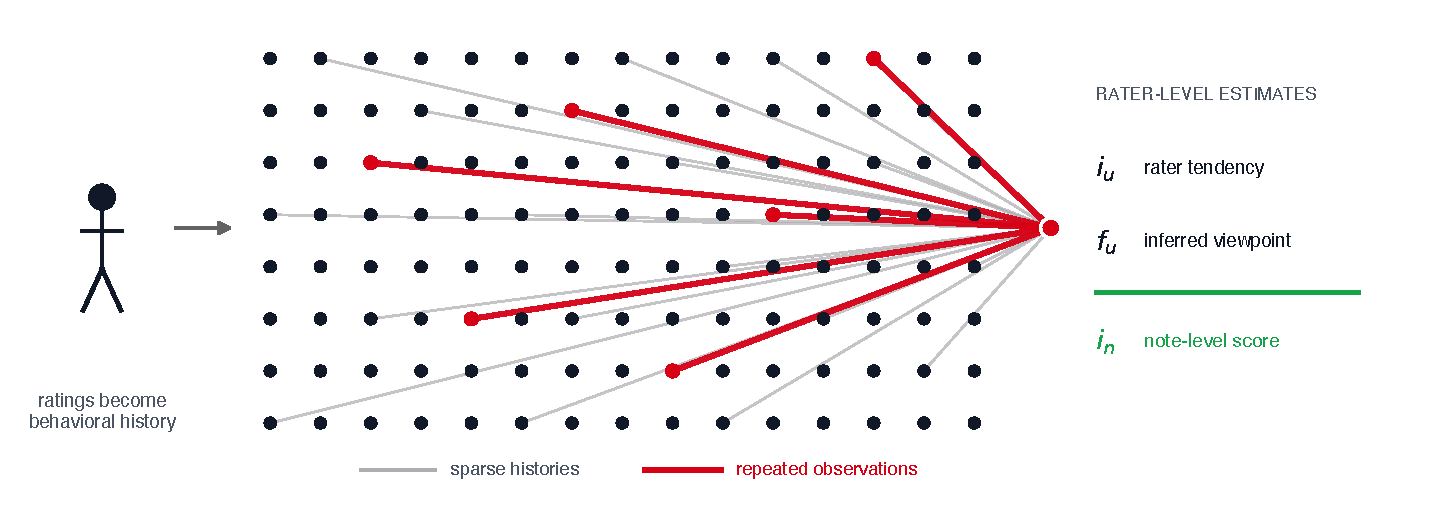
\includegraphics[width=0.93\textwidth]{../../figures/script_figures/07_fig1_cluster_signatures.pdf}
  \caption{Repeated participation gives a small set of highly active raters more
  leverage over the latent space fitted by matrix factorization. The model does
  not assign these users an explicit vote weight. Instead, their longer rating
  histories contribute more observations to the estimates of rater tendency
  ($i_u$) and viewpoint ($f_u$), which the pipeline uses before isolating the
  note-level score ($i_n$). The diagram is schematic and not drawn to scale.}
  \label{fig:rater-dominance-schematic}
\end{figure*}

\subsection*{The Algorithm in Practice: A Conceptual Map}
To illustrate how the mathematical components interact to deduce intent, we can map the algorithm's logic using three practical analogies:

\begin{enumerate}
    \item \textbf{The ``Amigo'' Knowledge Consumer ($f_u \cdot f_n$):}
    Imagine a highly partisan user who acts as a political ``amigo,'' a cheerleader for their ideological camp. Faced with a heavily biased note that flatters their own side, they vote ``Helpful'' without a second thought. The algorithm shrugs. It already computed the viewpoint match ($f_u \cdot f_n$) between this rater and this note, so the vote reads as \textit{``predictable cheerleading I could have called in advance.''} An approval that ideological alignment fully accounts for earns the note no extra credit: its helpfulness score ($i_n$) stays flat, and the note stays hidden \cite{wojcik2022birdwatch}.

    \item \textbf{Enemies Shaking Hands ($f_u \cdot f_n \approx 0$, $i_n$ spikes):}
    The reverse case is where the model earns its keep. Picture two raters at opposite poles of the spectrum, the kind who reliably pan whatever the other side applauds. When both of them, independently, mark the same note ``Helpful,'' viewpoint alignment can explain nothing: their agreement runs straight across the very axis used to predict their ratings. With that channel exhausted, the surplus has nowhere to land but $i_n$. The note registers as carrying something true enough to cross partisan lines \cite{buterin2023what}, and it surfaces.

    \item \textbf{The Hyperactive Minority ($f_u$ space distorted):}
    Both stories above assume the algorithm holds an honest map of where each rater sits in the latent space. It does not start with one; it draws the map from the rating record, and a few hands draw most of it. Think of a class graded on participation where the teacher keeps asking ``what does the class think?'' but the same handful of students answer every session; their voices quietly become the teacher's idea of the whole room. Community Notes inherits this distortion: a small, hyperactive, politically polarized minority supplies most ratings, so their behavior fixes where the axis of ``viewpoint'' lies and which votes look ``surprising'' \cite{nudo2026hyperactive}. That is what makes this third problem corrosive rather than additive. The first two diagnoses only hold if the map is honest; once a narrow crowd has drawn it, the ``enemies'' whose handshake looked so convincing may be two wings of the same overheated faction, and the bridge the model celebrates spans a gap most users were never placed on.
\end{enumerate}

\section{The Gap in Community Notes}
\label{sec:the_gap}

\subsection*{The Platform's Defense: Bridging}
X officially defends its algorithm using a ``bridging'' analogy \cite{xcommunitynotes2026ranking}. A note that draws support only from one side of the polarization axis is flagged as partisan and remains hidden. Visibility requires cross-group appeal: drawing positive ratings from raters the model places on opposite ends of the latent viewpoint dimension. Platform engineers argue this design prevents majority tyranny and resists coordinated manipulation by any single faction.

\subsection*{Why the Defense Does Not Hold}
The bridging claim rests on a prior step that undermines it. Before any cross-group comparison can take place, the formula described in Section~\ref{sec:how_cn_works} must situate every rater in a two-dimensional space of inferred identity. Two terms do this work:

$i_u$ collapses each rater to a single scalar, a leniency or strictness tendency estimated from their full history of votes. Whether a rater is critical because they apply high standards or because they systematically oppose certain content is not distinguishable from this number alone.

The viewpoint term $f_u \cdot f_n$ goes further: it pins each rater to a coordinate on an axis the model derives entirely from co-voting patterns. A ``Helpful'' rating is counted as cross-group signal only when the model could not have predicted it from that coordinate. Bridging, operationally, means ``this approval was surprising given where we placed this rater,'' not ``two independent communities both endorsed this note.''

The resulting action is intent inference rather than content evaluation. The algorithm asks not \textit{what} a note says, but \textit{who} tends to approve notes like this and whether an approver was the sort of person expected to do so. Sparse, unequal participation makes this inference even less reliable: when a small hyperactive minority supplies most of the votes that fix the latent axis, the coordinate system itself reflects their behavioral patterns, not the broader community's.

\subsection*{Evidence from Our Own Pipeline}

\begin{table}[h]
\centering
\small
\caption{Clustering stability across scale. Metrics reported after spectral AMG clustering; the 200k variant uses Method B vote-profile reassignment as the production partition. ``Hyperactive outlier'' reports the sub-population the algorithm separates at each scale and its median vote count relative to the main camps.}
\label{tab:scaleup}
\resizebox{\columnwidth}{!}{%
\begin{tabular}{lrrrp{4.2cm}}
\hline
Scale & ARI & Pearson & Discrim. & Hyperactive outlier \\
\hline
60k  & 0.989 & $-$0.69 & 86\% & absorbed (none) \\
150k & 0.977 & $-$0.65 & 83\% & 62 users ($\sim$7$\times$ more active) \\
200k\textsuperscript{$\dagger$} & 0.971 & $-$0.62 & 82\% & 64 users ($\sim$11$\times$) \\
210k & 0.969 & $-$0.62 & 81\% & 66 users ($\sim$12$\times$) \\
240k & 0.955 & $-$0.60 & 80\% & 60 + 1{,}431 users ($\sim$25$\times$) \\
250k & 0.997\textsuperscript{$\ddagger$} & --- & --- & degenerate: 249{,}933~/~67 \\
\hline
\end{tabular}}
\vspace{2pt}
\begin{flushleft}
\footnotesize
\textsuperscript{$\dagger$}Production setting; vote-profile reassignment gives Pearson $-$0.620, discriminating notes 81.4\%.\\
\textsuperscript{$\ddagger$}High ARI is an artefact: isolating the reproducible power-voter outlier as its own cluster maximizes stability while making the partition interpretively degenerate.
\end{flushleft}
\end{table}

To test whether scale resolves the participation problem, we ran a clustering ladder from 60k to 250k users across 19 variants. Table~\ref{tab:scaleup} reports the key metrics. Two findings emerge. First, the two-camp structure holds at every scale: bootstrap ARI remains above 0.95 and the between-camp Pearson correlation stays strongly negative throughout. Second, a hyperactive outlier reappears at every scale above 60k: a small group of power-voters, 7 to 25 times more active than ordinary raters, whom the algorithm consistently isolates as a distinct cluster. Larger samples do not dissolve this group; they rediscover it.

At 200k users the ladder reaches a stable equilibrium, found only after dozens of clustering and reassignment iterations. This is the production partition: it is the largest scale at which the two-camp structure remains clean and interpretable. Pushing to 250k breaks that equilibrium. The algorithm selects $k=2$ with a split of 249{,}933 versus 67, not because the two groups are genuinely comparable, but because isolating the reproducible power-voter outlier maximizes the bootstrap stability score. The partition is algorithmically optimal and interpretively useless.

\subsection*{The Problem, Stated}
Two failures sit beneath this gap, and only one is about data. The first is a matter of design: the algorithm profiles individuals instead of consulting communities, estimating whether a given rater's approval was predictable rather than whether the groups that genuinely disagree have each consented. This flaw is independent of sample size: with complete, perfectly balanced participation, the model would still be reading intent rather than evaluating cross-community consent. The second failure is empirical, and our ladder demonstrates it: the latent axis on which the entire bridging check rests is fixed by a hyperactive minority, so even the ``cross-group agreement'' the algorithm rewards is agreement across a distorted pair of poles. \citet{razuvayevskaya2025timeliness} measure this skew from the outside (the top 10\% of contributors produce 58\% of all notes), and our experiments confirm it from the inside, at every scale we can stably analyze. The gap is not a shortage of ratings. It is an aggregation rule that reads individual intent and then mistakes the most active raters' consensus for the community's.

\section{Learning from Divided Societies}
\label{sec:learning}

Section~\ref{sec:the_gap} left the production rule trying to bridge groups it
cannot name. If cross-group acceptability is going to be the display standard,
then the institutions built to decide across durable division are the natural
place to look for an aggregation rule. We draw the standard out first, then the
rules that honor it.

\subsection*{The Display Decision and Legitimacy}

Whether that gap matters, and how much, depends on what the display decision
ought to satisfy. Our answer is that when the platform aggregates many ratings
into a single show/hide decision, it makes a collective decision that requires
legitimacy. Three layers of argument support this.

First, display is a decision made in a collective name. A displayed note
attaches to the original post in the form ``readers added context,'' and the
platform thereby announces publicly, in the name of ``the community,'' that the
post is misleading. A decision made in a collective name and imposed on everyone
faces a minimal justification requirement: those affected should have reason to
accept the procedure that produced it \citep{klonick2018governors}. Second, no
user can opt out. A displayed note changes the informational environment of all
users, including the bloc that disagrees; no one can choose not to be affected by
it. Its binding force comes not from legal compulsion but from a non-excludable
change to a shared informational environment. Third, and most important here,
Community Notes itself already concedes this requirement. The mere existence of
the bridging criterion shows that the platform accepts that a note with
one-sided support should not be displayed; cross-ideological acceptability is
already its display standard, only realized in a latent-estimation form that
cannot express groups directly. Empirical evidence supports the instrumental
value of this commitment as well: relative to simple, context-free misleading
flags, community-style notes increase users' trust in fact-checking
\citep{drolsbach2024trust}. Asking about the legitimacy of the display decision
is therefore not the imposition of an alien political-philosophy requirement on a
recommender system; it makes explicit a commitment the system already holds,
turning it into checkable procedural criteria, and then asks which aggregation
rule should be used once that commitment is taken seriously.

The first two layers characterize the structure of the display decision: made in
a collective name, imposed on everyone, and borne jointly by all sides. This is
the structural signature of a constitutional decision that requires legitimacy.
The traditions that have thought longest, and at the highest cost, about how
groups who must live together under persistent cleavage make decisions of this
kind are the constitutional design of divided societies and, from the formal
side, social-choice theory. The limits of the borrowing should be drawn first:
the platform needs only a weakened version of this logic. Displaying a note does
not settle the normative design of state institutions, does not allocate state
power, and does not rely on legal compulsion. Accordingly, we appeal only to a
thin, procedural notion of legitimacy (the acceptability of a decision procedure
to the affected groups), and we borrow only the aggregation logic itself, not the
full normative theory of state legitimacy. For exactly this reason the
constitutional record is a conservative reference: it answers the heaviest
version of the problem, while the platform faces a lighter one.

\subsection*{Constitutional Design in Divided Societies}

Democracies that govern divided societies repeatedly decline to resolve
persistent disagreement by averaging over it; instead they institutionalize the
cleavage structure itself and set the validity condition of a collective
decision as concurrent acceptability across its component parts
\citep{lijphart1977democracy}. Table~\ref{tab:divided-societies} summarizes four
canonical cases: Switzerland's double-majority referendum requires both a
nationwide majority of voters and a majority of cantons \citep{lindermueller2021};
Belgium's consociational arrangements enforce parity between linguistic blocs
\citep{lijphart1977democracy}; Bosnia's post-Dayton constitution grants its
constituent peoples cross-group veto rights \citep{bieber2006}; and Northern
Ireland's parallel-consent rule requires that key Assembly decisions secure
support from both unionist and nationalist representatives
\citep{mcgarryoleary2009}.

\begin{table}[t]
\centering
\footnotesize
\renewcommand{\arraystretch}{1.25}
\begin{tabularx}{255pt}{@{}p{0.23\linewidth}X@{}}
\toprule
\textbf{System} & \textbf{Cross-community requirement} \\
\midrule
\mbox{\flagCH\ \textbf{Switzerland}} &
  Double majority: federal referenda require approval both by a
  national popular majority and by a majority of cantons
  \citep{lindermueller2021}. \\
\mbox{\flagBE\ \textbf{Belgium}} &
  Linguistic parity in the federal cabinet; major legislation
  requires parallel consent from Dutch- and French-speaking
  majorities in parliament \citep{lijphart1977democracy}. \\
\mbox{\flagBA\ \textbf{Bosnia}} &
  Vital-interest veto: any of the three constituent peoples
  (Bosniaks, Croats, Serbs) may block legislation deemed
  destructive to their community \citep{bieber2006}. \\
\mbox{\flagGB\ \textbf{N.\ Ireland}} &
  Parallel consent or weighted majority required for key
  Assembly votes, so decisions cannot pass without support from
  both the unionist and nationalist designations
  \citep{mcgarryoleary2009}. \\
\bottomrule
\end{tabularx}
\caption{Examples of constitutional systems that require cross-community or cross-regional approval.}
\label{tab:divided-societies}
\end{table}

The rules differ (some territorial, some linguistic, some ethno-national), but
they share one logic: these democracies observe that their societies contain
clusters defined by language, territory, ethnicity, or history, and treat the
existence of that cluster structure as politically meaningful in its own right.
This logic is also the source of non-compensatoriness. Each piece of legislation
subject to parallel consent is a self-contained decision settled in the present:
a key decision of the Northern Ireland Assembly requires unionist and nationalist
support at once, and support from one side cannot be traded for a victory on some
other bill. Acceptability must hold within that decision, across the groups,
simultaneously, with neither side dispensable, exactly the structure a
geometric-mean soft veto encodes, rather than a weighted average that offsets a
shortfall in one place with a surplus elsewhere. Power-sharing of this kind is
not costless: it can entrench group boundaries, empower communal elites, and
create veto points that obstruct governance
\citep{mcgarryoleary2009,schwartz2010,mcculloch2025}; we return to the limits of
the borrowing under limitations.

Seen through this lens, the carry-over to crowdsourced moderation is not to
estimate what each constituency latently thinks or wants (that would be quality
recovery displaced from notes to clusters) but to honor the cluster structure
itself, making each cluster's acceptability an independent condition for the
display decision on a single note.

\subsection*{Proportional and Representative Social Choice}

The constitutional record is qualitative; social-choice theory gives the same
logic from the formal side, and adds precision the constitutional record cannot
supply directly. The proportionality literature holds that a legitimate
collective decision should remain responsive to the distinct constituencies
rather than collapsing them into a single pooled electorate
\citep{peters2019proportionality}, and has been extended to participatory
budgeting and other multi-stakeholder settings \citep{peters2021proportional}.
Approval-based proportional representation makes the same point at the level of
axioms: justified representation and its stronger variants require that
sufficiently large cohesive coalitions not be washed out by majority aggregation
\citep{aziz2015justified,sanchez2017proportional}. Most directly relevant is
Qiu's formalization of \emph{representative social choice}
\citep{qiu2025representative}, which targets exactly the setting where
constituencies must be inferred from behavior rather than given ex ante: the
platform's situation, and the basis in the literature for the behavioral-recovery
criterion we state below.

In its problem structure, Community Notes corresponds to a repeated single-item
acceptance setting: for each note, the question is whether it clears a cross-group
acceptability bar. Repeated accept/reject decisions of this kind are the object
of the fair public decision-making literature
\citep{conitzer2017fair,lackner2020perpetual,skowron2022proportional}. Unlike
that literature, which places fairness at the sequential level (a constituency
outvoted on one issue can be compensated by influence on later ones), the display
decision is an unexitable individual act made in the community's name. There is
no sequence across which to amortize, so acceptability must hold within each
note, which reinforces the non-compensatoriness already obtained from parallel
consent.

Combining the two literatures yields three conclusions that bear directly on the
design criteria: (i) the validity condition of a decision should be the
\emph{concurrent} acceptability of the constituencies, not the average
acceptability of a pooled total (constitutional record and proportionality);
(ii) constituencies cannot be given ex ante on the platform and must be inferred
from behavior (representative social choice); and (iii) because the display
decision is unexitable and cannot be amortized across decisions, acceptability
must hold \emph{non-compensatorily} within a single note, across the
constituencies (parallel consent and within-decision fairness). We state these
three, together with the symmetry requirement they imply, as four operational
criteria in the next section.

\section{Cross-Constituency Aggregation}
\label{sec:cca}

\subsection*{Design Criteria}

The legitimacy argument and the three conclusions above narrow the design space
to a few requirements on any rule that decides under structured disagreement. We
state four, each answering to one component of the CCA rule. The behavioral rater
clusters are not nations in the constitutional sense, and we do not claim they
hold such groups' normative standing; the criteria are \emph{weakened}
aggregation requirements, drawn from the institutional and social-choice record
and adapted to platform governance. Each criterion is stated below with the
institutional source it is drawn from and the CCA component that discharges it,
and Table~\ref{tab:principles-map} collects the same mapping at a glance.

\textbf{P1 (Presence).} No display decision may be made while any constituency is
absent; missing representation must not be convertible into apparent consensus.
\emph{(Source: quorum and double-majority requirements, as in Switzerland's
double majority; the precondition of concurrent acceptability. CCA component:
each constituency must contribute at least three raters.)}

\textbf{P2 (Non-compensation).} One constituency's strong rejection cannot be
offset by another's enthusiasm; acceptability must hold within each constituency,
not merely in the cross-constituency average. \emph{(Source: mutual veto and
parallel consent, as in Bosnia and Northern Ireland; acceptability must hold
within a single note across the constituencies, ruling out compensation. CCA
component: geometric-mean aggregation, a soft veto.)}

\textbf{P3 (Symmetry).} Constituencies enter the decision on equal footing,
independent of relative size or rating activity. \emph{(Source: parity rules, as
in Belgium; concurrent acceptability treats the constituencies as equal
conditions. CCA component: the aggregator is symmetric in its arguments and
operates on within-constituency approval rates rather than raw counts.)}

\textbf{P4 (Behavioral recovery).} Since no ex-ante partition of raters exists,
constituencies must be recovered from observed behavior transparently and
reproducibly. \emph{(Source: representative social choice, conclusion (ii) above;
no direct constitutional analogue; this is where the platform setting departs
from constitutional design. CCA component: spectral clustering on co-rating
similarity, with stability diagnostics.)}

\newcolumntype{Y}{>{\raggedright\arraybackslash}X}
\begin{table}[t]
  \centering
  \footnotesize
  \setlength{\tabcolsep}{4pt}
  \renewcommand{\arraystretch}{1.25}
  \begin{tabularx}{\columnwidth}{@{}YYYY@{}}
    \toprule
    \textbf{Principle} & \textbf{Requirement} & \textbf{Source (\S\ref{sec:learning})} & \textbf{CCA component} \\
    \midrule
    \textbf{P1} Presence & No absent constituency & Double majority (CH) & Coverage rule \\
    \addlinespace[2pt]
    \textbf{P2} Non-compensation & No cross-bloc offsetting & Mutual veto (BA, NI) & Geometric mean \\
    \addlinespace[2pt]
    \textbf{P3} Symmetry & Equal footing, any size & Parity rules (BE) & Symmetric aggregator \\
    \addlinespace[2pt]
    \textbf{P4} Behavioral recovery & Blocs inferred, not labeled & Representative social choice & Spectral clustering \\
    \bottomrule
  \end{tabularx}
  \caption{The four design criteria at a glance: each principle (P1--P4), the
  requirement it places on the display decision, the divided-society or
  social-choice source it is drawn from (Section~\ref{sec:learning}), and the
  CCA component that discharges it.}
  \label{tab:principles-map}
\end{table}

\subsection*{Rule Definition}

The rule is stated over two behavioral constituencies, recovered from co-rating
structure by the clustering described in Section~\ref{sec:approach}. We
operationalize the criteria in four steps: cluster raters into $K=2$ behavioral
constituencies by co-rating similarity (P4); for each note, compute its approval
rate within each constituency separately (P3); aggregate the two per-constituency
approvals with a geometric mean (P2); and select a note only when that mean
clears the display threshold and both constituencies are present (P1).

Let $a_{ic}$ be note $i$'s approval rate inside constituency $c$, the share of
helpful ratings among that constituency's ratings of the note. Writing $H_{ic}$
and $N_{ic}$ for the helpful and total ratings note $i$ receives from
constituency $c$,
\begin{equation}
a_{ic} =
\begin{cases}
H_{ic}/N_{ic}, & N_{ic} > 0,\\
0.5, & N_{ic} = 0.
\end{cases}
\end{equation}
The $0.5$ fallback marks abstention, not endorsement: a constituency that has
never rated the note casts no vote. Presence (P1) forbids that abstention from
ever standing in for support, so the fallback alone never selects a note; both
constituencies must contribute at least three raters before the note is scored
at all. For a note that clears this coverage bar, the cross-constituency score is
the geometric mean
\begin{equation}
    C_i = \sqrt{\max(a_{i1},\epsilon)\,\max(a_{i2},\epsilon)},
    \label{eq:cca-score}
\end{equation}
with $\epsilon = 10^{-6}$ guarding against a hard zero. A note is CCA-selected
when $C_i \geq 0.5$ and the coverage requirement is met; when Community Notes
does not already display it, the selected note enters the CCA rescue pool.

The geometric mean is the minimal aggregator that meets P2 and P3 at once:
symmetric in its arguments, increasing in each on $(0,1]^2$, and collapsing to
zero as either rate does. A plain minimum would also veto, but it ignores the
stronger side entirely; a weighted average would let one side's surplus offset
the other's shortfall, which P2 forbids. The mean carries a further robustness
worth naming: if one constituency scores systematically more strictly, approving
the same notes at lower rates, it rescales every note by roughly the same factor,
which the display threshold absorbs uniformly and which leaves the order of notes
near the display line unchanged. The direction of construction is the point: the rule is the product of the four criteria, not reverse-engineered to fit the data.
We do not claim the geometric mean is the unique function with these properties;
for a rule aimed at improving the display decision, what is needed is that the
chosen rule delivers them.

\subsection*{Objections and Scope}

Reading the production model against these criteria, the gap between its
commitment and its realization can be stated precisely. Eq.~\eqref{eq:cn-model}
does contain a kind of counterpart to P2: the bridging term penalizes support
drawn from only one end of the spectrum, crediting a note's helpfulness ($i_n$)
only for approval that the viewpoint match $f_u \cdot f_n$ cannot explain. But the
constituency form of P2, that acceptability hold separately within each group,
cannot be stated in the model, because groups are not model objects. P1 has no
counterpart at all: pooled estimation has no notion of ``a group being absent,''
and raters from a single group can wholly dominate the estimate of $i_n$. P3 is
likewise absent: a larger or more active bloc simply contributes more terms to the
loss. The polarization safeguard conflicts directly with P2, discounting notes on
\emph{polarizing issues} rather than notes with \emph{one-sided support}, so it
can veto a note that both groups accept. The reliability-weighted extension
\citep{goyal2026qsmf} inherits the same representational structure. This is the
design failure of Section~\ref{sec:the_gap}: the rule reads individual intent
where the criteria ask for community consent.

Our own rule invites objections in turn. The first concerns P4: by what right do
algorithmically recovered clusters acquire the standing of constituencies? In
constitutional regimes that standing comes from history, language, or identity; on
the platform none of these is available, so it can come only from the structure of
the disagreement itself. We require three things of a partition before it counts.
It must persist under subsampling and across sample sizes, which the clustering
ladder of Section~\ref{sec:the_gap} confirms with a bootstrap ARI above 0.95 at
every scale. Each side must be large enough that cross-constituency agreement is a
demand on two real publics rather than statistical noise; our two constituencies
each hold tens of thousands of raters, while the 64-user power-voter cluster the
diagnostics keep surfacing is denied standing precisely because it fails this
test. And the two must reach different verdicts on a large share of notes; about
81\% of evaluated notes fall on the discriminating side of the partition. A
partition meeting all three is not an arbitrary artifact but the lines along which
acceptance and rejection actually run. The standing is conditional: when rating
behavior no longer shows a stable cluster structure, CCA's precondition fails and
pooled estimation regains its warrant.

An immediate worry follows: once the behavioral partition is reduced to two
classes, is it not the same as splitting the model's one-dimensional ideology axis
in two at the sign of $f_u$? Even when both are binary, they are different objects.
The $f_u$ split requires choosing a cut point on a single jointly fitted line; the
behavioral split comes from the full co-rating similarity structure, and its
boundary need not correspond to any threshold on that line. Topic-level
diagnostics already point away from coincidence: neither constituency is
uniformly more approving across issues, while the between-camp correlation stays
strongly negative throughout the clustering ladder (Table~\ref{tab:scaleup}).
There is also a procedural reason to keep them apart:
$f_u$ is an internal quantity estimated by the very model under audit, and using
the audited rule's own instrument to delineate the parties would be improper,
whereas the behavioral constituencies are recovered from raw rating behavior
independent of that rule.

A second worry concerns rescue itself: why should a note that fails the platform's
cross-ideological test regain value under cross-constituency consent, when the two
are two statements of the same intuition? They are, and that is precisely why the
rescue pool is well defined: it is the set on which the two operationalizations of
one consent standard \emph{disagree in verdict}. Three mechanisms can produce that
disagreement. (a) The polarization safeguard may conflate ``the issue is
contentious'' with ``the support is one-sided,'' suppressing notes on contested
issues that both sides in fact accept. (b) A single spectrum may fail to express
the real bloc structure: the model places each rater at a point on the axis,
whereas the actual blocs are multidimensional, organized by which issues each
group attends to and what evidence it accepts. Two raters at opposite ends of the
axis need not belong to different blocs, and two placed nearby need not share one,
so support that bridges along the axis and support that travels across blocs may
not coincide. (c) The strongly regularized latent estimate is conservative and
sample-inefficient by construction \citep{goyal2026qsmf}, and observable
cross-group support need not produce the residual pattern that matrix
factorization rewards. CCA therefore does not overturn the platform's verdict on
some shared question; it indicates that a portion of those verdicts may be
artifacts of the realization rather than rulings of the consent standard itself.

These criteria are the requirements of a defensible rule under structured
disagreement, not a claim that the platform's rule is illegitimate in all
settings. When rater disagreement is unstructured noise around a shared quality
signal, pooled latent-quality estimation is well warranted; it is the persistence
of behavioral blocs, documented in Section~\ref{sec:the_gap}, that makes the
cross-constituency question the right one here.

\section{Approach}
\label{sec:approach}

\subsection{Data and Pipeline}

The empirical pipeline follows the repository's active 200k Representative
setup. Active raters are clustered from rating behavior, downstream analysis
uses Method-B reassigned clusters, and note-level outcomes are evaluated on the
canonical production paths documented in the repository README.

\begin{figure}[h]
  \centering
  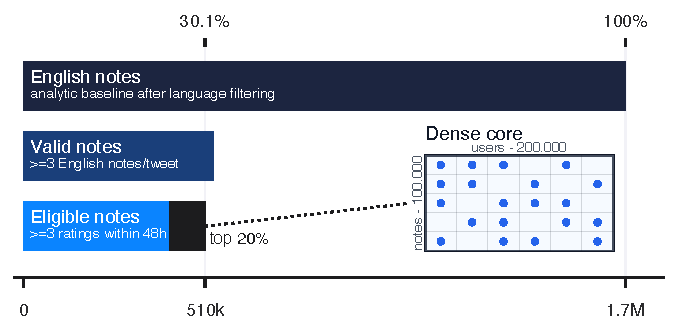
\includegraphics[width=\columnwidth]{../../figures/script_figures/07_fig3_pool_and_topics.pdf}
  \caption{Construction of the analytical sample. Starting from 1.7M English
  notes, we keep notes on tweets with at least three English notes and at least
  three eligible helpful/not-helpful ratings cast within 48 hours of creation,
  yielding 510k eligible notes; from these we select a 100k-note dense slice
  (about the top 20\% by rating volume) and retain 200k active raters for
  clustering.}
  \label{fig:dataset-construction}
\end{figure}

\subsection{Validation}

Candidate rescued notes should be validated separately from the aggregation
step. The validation layer should ask whether a note is sourced, factual,
relevant to the original post, and useful enough to justify surfacing. This
keeps the social-choice rule and the content-quality judgment analytically
separate.

\section{Results}
\label{sec:results}

This section will report the size of the rescue pool, the share of notes that
would become visible under cross-constituency aggregation, validation outcomes,
and the topical distribution of rescued notes.

\begin{figure}[h]
  \centering
  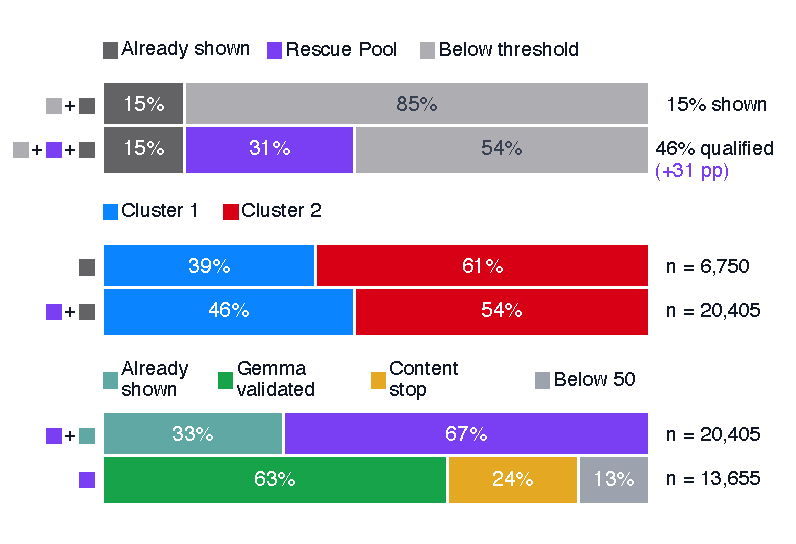
\includegraphics[width=\columnwidth]{../../figures/script_figures/07_fig5_rescue_panels.pdf}
  \caption{Cross-constituency aggregation expands the qualified set and validates
  hidden candidates. Among 44,722 representative-picked notes, 20,405 meet the
  CCA threshold: 6,750 are already shown and 13,655 form the hidden rescue pool.
  Gemma validates 8,558 candidates; 3,279 stop at the content screen, and 1,818
  receive rescue-worthiness scores below 50.}
  \label{fig:rescue-panels}
\end{figure}

\begin{table}[t]
\centering
\small
\begin{tabular}{l r}
\toprule
\textbf{Note set} & \textbf{Count} \\
\midrule
Representative-picked note universe & 44{,}722 \\
CN shown within representative picks & 6{,}832 \\
CCA rescue pool & 13{,}655 \\
CCA visible total & 20{,}487 \\
\midrule
CCA rescued after Gabriel validation & 3{,}896 \\
Opinion/speculation in rescue pool & 3{,}610 \\
Other excluded in rescue pool & 6{,}149 \\
\bottomrule
\end{tabular}
\caption{Representative-picked notes shown by Community Notes versus the CCA
rescue pool and its validation outcome.}
\label{tab:rep-cn-overlap}
\end{table}

\section{Discussion}

The discussion will connect the empirical results to platform legitimacy,
social choice under disagreement, and the limits of crowdsourced moderation.

One development is already visible in the platform's own direction. In November
2025 X began piloting a final-scoring model that aggregates helpfulness through a
geometric mean of helpfulness rates across the rater-factor spectrum
\citep{xcommunitynotes2026ranking}, the soft-veto logic of CCA, adopted inside
the production pipeline but still organized along one fitted axis. The step CCA
formalizes is the obvious next one: take that geometric mean over behaviorally
recovered constituencies, each required to be present, rather than over points
on an estimated ideology line.

\section{Limitations}

This section will state where the proposed rule is conservative and where it may
fail. Anticipated limitations include the two-camp assumption embedded in the
current clustering setup, the fact that behavioral constituencies do not map
cleanly onto ideological or demographic categories, the reliance on LLM-based
validation in the second stage, and the conservative effect of the
minimum-coverage requirement on rescue pool size.

\section{Conclusion}

The paper will argue that visibility decisions in crowdsourced fact-checking
should preserve the structure of disagreement instead of compressing it into a
single pooled consensus score too early.

\bibliographystyle{plainnat}
\bibliography{references}

\end{document}
